\documentclass[12pt]{l4dc2023}
\usepackage{amsmath,amssymb}

\usepackage{booktabs}
\usepackage{graphicx}
% The following packages will be automatically loaded:
% amsmath, amssymb, natbib, graphicx, url, algorithm2e

\title{On The Formally Verifying Congestion Control Algorithms Behavior}
\usepackage{times}
% Use \Name{Author Name} to specify the name.
% If the surname contains spaces, enclose the surname
% in braces, e.g. \Name{John {Smith Jones}} similarly
% if the name has a "von" part, e.g \Name{Jane {de Winter}}.
% If the first letter in the forenames is a diacritic
% enclose the diacritic in braces, e.g. \Name{{\'E}louise Smith}

% Two authors with the same address
% \coltauthor{\Name{Author Name1} \Email{abc@sample.com}\and
%  \Name{Author Name2} \Email{xyz@sample.com}\\
%  \addr Address}

% Three or more authors with the same address:
% \coltauthor{\Name{Author Name1} \Email{an1@sample.com}\\
%  \Name{Author Name2} \Email{an2@sample.com}\\
%  \Name{Author Name3} \Email{an3@sample.com}\\
%  \addr Address}

% Authors with different addresses:
\author{%
 \Name{Behrooz Farkiani} \Email{b.farkiani@wustl.edu}\\
 \addr 1 Brookings Dr., Washington University in St. Louis, MO, 63130 
}

\begin{document}

\maketitle
\begin{abstract}
Congestion control algorithms play a vital role in the efficiency of communication over the Internet. However, the primary way to analyze their performance has traditionally been through extensive simulation and/or emulation. This work investigates the use of formal methods to analyze the behavior of AIMD and BBR congestion control algorithms based on the paper "Toward Formally Verifying Congestion Control Behavior." The authors found that AIMD can exhibit surprising behavior, where premature loss leads to a very small congestion window even when the network has a noticeably large bottleneck buffer. They also analyzed AIMD and proposed a steady-state bound defined in terms of the congestion window and loss limits. For BBR, they observed that it can achieve very low utilization, which is harmful to its performance.

In this study, I investigated the authors' implementation in detail and documented the behavior of the network and congestion control algorithms. I identified and questioned several aspects of the original implementation and proposed enhancements. I compared the original implementation with my enhancements. My modifications achieved better real-world results while still preserving the surprising behavior of AIMD and the low utilization reported for BBR. Additionally, I found that the proposed steady-state bounds are not valid and can be violated.

\end{abstract}

\begin{keywords}%
  Congestion Control, BBR, AIMD, SMT, Formal Verification, Z3
\end{keywords}

\section{Introduction}

Efficient end-to-end data delivery must (1) prevent a sender from congesting the network and (2) enforce limits on incoming traffic to avoid capacity overflow while improving reliability and availability. The former is embodied in \emph{congestion-control} algorithms and the latter in \emph{flow-control} algorithms. The paper I am discussing here, \emph{Toward Formally Verifying Congestion Control Behavior} (\cite{CCAC}), focuses on congestion control and proposes a tool named \emph{CCAC} that uses formal-verification tools to study congestion-control algorithms' behavior.  
Traditional evaluation relies on extensive simulations or live A/B tests, which are time and resource-intensive. This work instead uses formal verification to model both the network path and the sender's control logic as an SMT problem, allowing Z3 to prove performance bounds or generate concrete counter-examples.

The network between sender and receiver is shared among multiple senders; for instance, it can be an interconnection of independent networks such as the Internet. The network has finite capacity and may carry traffic from many senders simultaneously.  
If the aggregate input rate exceeds the link's capacity, \emph{congestion} occurs, leading to buffer overflow and packet loss. Senders must therefore regulate their sending rate to avoid both network congestion and receiver overload. Although receivers also have finite buffers, CCAC does not model receiver-side flow control. There exist many congestion-control algorithms in the literature (\cite{jiang_when_2021}); CCAC models AIMD (\cite{aimd}), BBR (\cite{bbr}), and Copa (\cite{copa}), and we focus here on AIMD and BBR as they are most widely deployed.

CCAC assumes a reliable, in-order byte stream between sender and receiver. The sender partitions data into segments (\emph{packets}) of arbitrary size, each labeled with a unique byte-sequence number. When the receiver obtains all bytes up to sequence number $n$, it sends a \emph{cumulative ACK} of value $n{+}1$. If later packets arrive out of order, the receiver can emit \emph{duplicate ACKs}, each carrying the same ACK number.                                                                                                                                                                                                          
For example:
\begin{itemize}
  \item Bytes 10-99 arrive correctly, so the receiver ACKs~100.
  \item Bytes 100-199 are lost, but then bytes 200-299, 300-399, and 400-499 arrive.
  \item The receiver cannot advance its ACK beyond 100, so it emits three duplicate ACKs with value~100.
\end{itemize}
Upon receiving three duplicate ACKs, the sender's fast-retransmit mechanism resends the missing segment.  
Separately, each packet starts a retransmission timer: if its ACK does not arrive before timeout, the sender assumes loss and retransmits.

CCAC combines the path and receiver into a single \emph{path-server} model. Thus the formalization comprises:
\begin{enumerate}
  \item \emph{Sender equations}, which specify how the sender adjusts its congestion window $cwnd(t)$ in response to network behavior, ACKs, and losses from the path-server.
  \item \emph{Path-server equations}, which enforce capacity, buffering, jitter, and waste constraints on incoming traffic.
\end{enumerate}

When traffic flows, it experiences various delays, including \emph{propagation delay} and \emph{queueing delay}. CCAC uses a simplified path-server as shown in Figure \ref{fig:tb}. It assumes network capacity depends on a bottleneck link with a fixed capacity $C$ (bytes/s).  
The network also has a round-trip propagation delay $R_{m}$ (s). Capacity is enforced via a \emph{token bucket} that generates tokens at rate~$C$ and stores them in a token-bucket queue. The token queue has a limited capacity~$K$, and tokens generated when this capacity is filled will be wasted. In addition, new tokens can arbitrary be \emph{wasted} if the token-queue length exceeds the packet-queue length, ensuring that waste does not reduce service capacity. This allows jitter in service rate. In addition, the path has a FIFO packet queue. Arrivals first enter this queue and are served as tokens allow. When $X$ bytes of packets arrive:

\begin{itemize}
  \item In the absence of arrivals, the bucket accumulates tokens up to $K$
  \item Admitted packets may be delayed up to $D$ seconds before service, simulating burstiness, ACK aggregation, MAC-layer scheduling, etc.
  \item Admitted tokens cannot remain unused longer than $D$, so $K=C\cdot D$ bounds the maximum burst.
\end{itemize}

\begin{figure}[htbp]
    \centering
    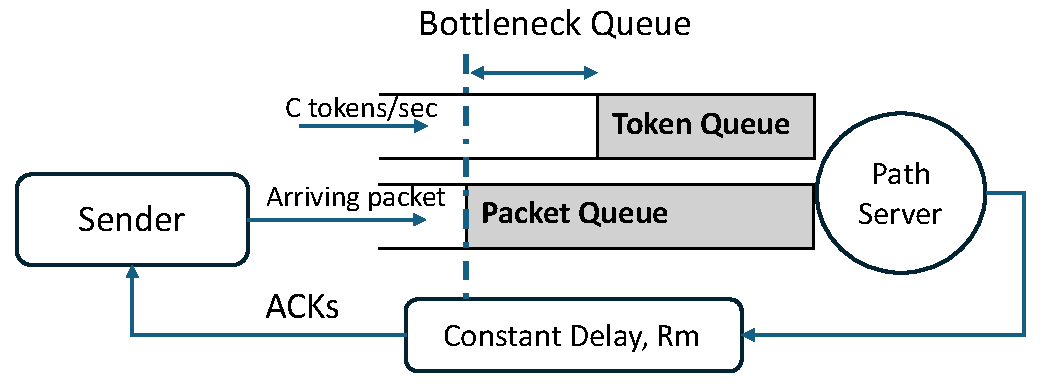
\includegraphics[width=0.75\linewidth]{tb.pdf}
    \caption{CCAC's Path-server model}
    \label{fig:tb}
\end{figure}

The difference between what arrives and what is served forms the \emph{bottleneck queue}. This queue has a finite capacity~$B$; if the backlog exceeds $B$, overflow occurs and packets are lost. The sender regulates the amount of traffic it send to the network via the congestion window $cwnd(t)$, which caps the \emph{in-flight} data (bytes sent but not yet acknowledged or declared lost). Whenever $\mathrm{inflight}<cwnd$, the sender may inject additional data up to the window limit. Different congestion control algorithms adjust $\mathrm{cwnd}$ in distinct ways; for example, based on duplicate ACKs, timeouts, or measured delivery rates, and CCAC's simplified model captures these behaviors as we describe in later sections. 

The paper studies a single sender-receiver flow, simplified versions of congestion-control algorithms, and worst-case network behavior. Its main contributions are:
\begin{itemize}
  \item Modeling the path-server and congestion-control logic as an SMT instance, and using a set of SMT queries to analyze congestion-control behavior.
  \item Showing that AIMD can incorrectly reduce its congestion window due to buffer overflow even when buffer is large. This phenomenon is referred to as \textit{surprising behavior} in AIMD.
  \item Proposing a new steady-state bound for AIMD.
  \item Demonstrating that BBR's utilization can drop to very low levels.
\end{itemize}

My analysis and contributions address the following:
\begin{itemize}
  \item I describe and validate the SMT implementation of the model, filling in details omitted from the original paper.
  \item I propose four enhancements (\textit{fixes}) to the model and its queries.
  \item I demonstrate, using the enhanced model, that the proposed steady-state bounds for AIMD do \emph{not} always hold.
\end{itemize}

The remainder of the paper is organized as follows. Section \ref{network} describes the path-server model as implemented in SMT. Section \ref{aimdSection} presents the AIMD congestion control algorithm and its implementation, and Section \ref{BBR} describes BBR. Section \ref{enhancements} discusses the proposed enhancements, and Section \ref{evaluation} presents the evaluation results of the original implementation and the enhanced model. Finally, Section \ref{conclusion} concludes the paper.

  
\section{Modeling of Network and Algorithms} \label{network}

This section first describes the network model, and then investigates how AIMD and BBR are implemented. Notations are shown in Table \ref{tab:notation}. 

\begin{table}[ht]
\centering
\begin{tabular}{@{}ll@{}}
\toprule
\textbf{Symbol} & \textbf{Description} \\
\midrule
\(A(t)\) & Cumulative bytes arrived at the path-server by time \(t\). \\
\(S(t)\) & Cumulative bytes served by the path-server (i.e., ACK bytes sent toward the sender) by time \(t\). \\
\(L(t)\) & Cumulative bytes lost by the path-server by time \(t\). \\
\(W(t)\) & Cumulative tokens wasted by the path-server by time \(t\). \\
\(Q(t)\) & Packet queue length at time \(t\), \(Q(t)=A(t)-L(t)-S(t)\). \\
\(A_f(t)\) & Cumulative bytes sent by the sender (per-flow) by time \(t\). \\
\(L_f(t)\) & Cumulative bytes lost (per-flow) by time \(t\). \\
\(Ld_f(t)\) & Cumulative losses detected by sender (dupacks/timeouts) by time \(t\). \\
\(S_f(t)\) & Cumulative bytes served (per-flow) by time \(t\). \\
\(r_f(t)\) & Pacing rate (bytes per timestep) at time \(t\). \\
\(\mathrm{Inflight}(t)\) & Sender's in-flight bytes at time \(t\), \(\mathrm{Inflight}(t)=A_f(t)-Ld_f(t)-S_f(t-R_m)\). \\
\(\mathrm{timeout}(t)\) & Boolean: sender timeout at time \(t\). \\
\(T(t)\) & Token queue length at time \(t\), \(T(t)=C\cdot t - W(t) - S(t)\). \\
\(C\) & Fixed bottleneck link capacity (bytes per timestep). \\
\(D\) & Maximum per-packet jitter (timesteps). \\
\(\beta\) & Buffer capacity (bytes). \\
\(\alpha\) & Additive-increase increment. \\
\(R_m\) & Round-trip propagation delay (timesteps). \\
\(\mathtt{buf\_min},\,\mathtt{buf\_max}\) & Minimum/Maximum buffer thresholds. \\
\(\mathrm{dupacks}\) & Duplicate-ACK threshold for loss detection. \\
\(\mathrm{cwnd}_f(t)\) & Congestion window (bytes) of flow f at time \(t\). \\
\(T\)& Evaluation duration. \\
\bottomrule
\end{tabular}
\caption{Notation used in the CCAC path-server SMT model.}
\label{tab:notation}
\end{table}

\subsection{Network model}
The network is modeled as a token-bucket filter with maximum service rate $C$, up to $D$ timesteps of per-packet delay, and a fixed round-trip propagation delay of $R_m$.

\subsubsection{Token-bucket balance}
\[
T(t) \;=\; C \cdot t \;-\; W(t) \;-\; S(t)
\]

\subsubsection{Network queue length}
\[
Q(t) \;=\; A(t) \;-\; L(t) \;-\; S(t)
\]

The difference between Q(t) and T(t), packet queue and token bucket queue, will be held at bottleneck queue. Loss happens when bottleneck queue exceeds bottleneck queue capacity. 

\subsubsection{Monotonicity (for \(1\le t<T\)):}
\[
\begin{aligned}
A_f(t)&\ge A_f(t-1), & L_f(t)&\ge L_f(t-1),\\
S_f(t)&\ge S_f(t-1), & Ld_f(t)&\ge Ld_f(t-1),\\
W(t)&\ge W(t-1), & A_f(t)-L_f(t)&\ge A_f(t-1)-L_f(t-1).
\end{aligned}
\]
All cumulative quantities (arrivals, losses, service, and waste) must be non-decreasing.
\subsubsection{Initialization (at \(t=0\)):} \label{w}
\[
\begin{aligned}
\mathrm{cwnd}_f(0)&>0,\quad r_f(0)>0,\quad L_f(0)\ge0,\quad Ld_f(0)\ge0,\quad  S_f(0)&=0.
\end{aligned}
\]
As we see, the original implementation does not enforce wasted tokens W(t) to be non-negative.

\subsubsection{Total-flow relations (single flow):}
\[
A(t)=A_f(t),\quad L(t)=L_f(t),\quad S(t)=S_f(t).
\]

\subsubsection{Network capacity and queuing (for all \(0\le t<T\)):}
\[
\begin{aligned}
S_f(t)&\le A_f(t)-L_f(t),\\
C\,(t-D)-W(t-D)&\;\le\;S(t)\;\le\;C\cdot t - W(t).
\end{aligned}
\]
with \(W(t-D)\) replaced by \(W(0)\) if \(t<D\). Service rate must be less than or equal to effective input to the network. Service rate is also bounded by generated tokens that are not wasted from above. We need to also ensure that tokens remaining from D second ago that are not wasted must have been server. These two are service bounds. 

\emph{Wastage constraint:}
\[
W(t)>W(t-1)\;\Longrightarrow\; A(t)-L(t)\le C\,t - W(t) 
\]
The above condition ensures the wastage allows only if effective input $A(t)-L(t)$ is less than serving capacity. 

\emph{Buffer-minimum:}
\[
L(t)>L(t-1)\;\Longrightarrow\;
A(t)-L(t)\ge C\,(t-1)-W(t-1)+\mathrm{buf\_min}.
\]
Loss happens only when $Q(t)-T(t-1)>\beta$, i.e., difference between packet queue and token queue exceeds the bottleneck buffer size. We see authors used $T(t-1)$ instead of $T(t)$ because loss means we inserted data when token was not available, i.e., tokens were not generated at the same pace as we inserted data. 
 
\emph{Buffer-maximum:}
\[
A(t)-L(t)\;\le\;C\,t - W(t) + \mathrm{buf\_max}.
\]

\subsubsection{Loss detection (for all \(0\le t<T\) and \(dt\) with \(t-R_m-dt\ge0\)):} \label{loss}

Define

\[
\mathrm{detectable}(t,dt)\;:\;
A_f(t-R_m-dt)-L_f(t-R_m-dt)+\mathrm{dupacks}
\;\le\;S_f(t-R_m).
\]
Loss is detectable when three duplicate acks arrive. Assume $dt=0$ and the formula above would be

\[
\mathrm{detectable}(t,dt)\;:\;
A_f(t-R_m)-L_f(t-R_m)+\mathrm{dupacks}
\;\le\;S_f(t-R_m).
\]
Suppose $t=4$, $R_m=1$, and $\mathit{dupacks}=3$. At time $t-R_m=3$, let $A_f(3)=12$ and $L_f(3)=2$. Then $A_f(3)-L_f(3)=10$, the count of in-order bytes delivered. To detect the two lost bytes among those 12, the sender needs $10+\mathit{dupacks}=13$ ACKs. Hence, if by time 3 the path-server has served at least 13 bytes (so $S_f(3)\ge13$), those 13 ACK-bytes arrive at the sender at $t=4$ because of propagation delay, and the code sets \texttt{detectable} to true.

Whatever packets arrive may experience queueing delay before being served.  Since the loss has already occurred in the past, CCAC introduces an index \(dt\) to scan all candidate loss epochs \(t - R_m - dt\) and determine the earliest time at which the sender has received enough duplicate ACKs to detect that loss.

\[
\begin{aligned}
\neg\mathrm{timeout}(t)\land \mathrm{detectable}(t,dt)
&\implies Ld_f(t)\ge L_f(t-R_m-dt),\\
\neg\mathrm{timeout}(t)\land \neg\mathrm{detectable}(t,dt)
&\implies Ld_f(t)\le L_f(t-R_m-dt).
\end{aligned}
\]

These constraints ensure that, if no timeout occurs at time \(t\) and a loss is detectable after a delay offset $dt$, then the cumulative detected-loss counter $Ld_{f}(t)$ must be at least the actual cumulative loss $L_f(t-R_m-dt)$.  Conversely, if the loss is not detectable, \(Ld_{f}(t)\) cannot exceed $L_f(t-R_m-dt)$.  Since both \(Ld_{f}\) and \(L_f\) are cumulative, this encodes a superset of possible real-world behaviors.

Note that the model does not preclude spurious loss detections; it permits \(Ld_{f}(t)>0\) even when no actual loss has occurred.  

\emph{Timeout definition:}
For \(t< R_m\): $\mathrm{timeout}(t) = \mathsf{false}.$ For \(t \ge R_m\): 
\[
\mathrm{timeout}(t) \;=\; 
\bigl(S_f(t-R_m) < A_f(t-1)\bigr)
\;\wedge\;
\bigl(S_f(t-R_m) = A_f(t-R_m) - L_f(t-R_m)\bigr).
\]
Timeout at time \(t\) is triggered when there are still outstanding bytes (i.e.\ \(S_f(t-R_m) < A_f(t-1)\)) and the service delivered at \(t-R_m\) exactly equals the effective arrivals up to that point (\(A_f(t-R_m) - L_f(t-R_m)\)).  
As the authors note, this \textit{magical} RTO logic does not correspond to real-world timers, and implementing it in this way is strange. 

\emph{Effects on detected loss:}
\[
\mathrm{timeout}(t)\;\Longrightarrow\; Ld_{f}(t) = L_f(t),
\]
\[
L_{d,f}(t)\;\le\;L_f(t-R_m).
\]
On timeout, the detected-loss counter \(Ld_{f}(t)\) jumps to the current cumulative loss \(L_f(t)\). Moreover, it ensures detected losses never exceed the actual losses that occurred at least one RTT earlier.

\subsubsection{8. CWND and arrival rate (for \(t\ge R_m\)):}
The congestion window \(\mathrm{cwnd}_f(t)\)  upper-bounds the amount of new data the sender may inject. In the CCAC model, the formula
\[
A_w = S_f(t - R_m) \;+\; Ld_{f}(t) \;+\; \mathrm{cwnd}_f(t)
\]
encodes the usual \emph{window-limited} bound on how many bytes the sender may have cumulatively sent by time \(t\). Concretely, \(S_f(t - R_m)\) is the total bytes the sender has \emph{already} seen acknowledged (via ACKs that departed the path-server at \(t-R_m\)).
\(Ld_{f}(t)\) is the total bytes the sender has \emph{detected} as lost up through time \(t\) that sender needs to resend, and $\mathrm{cwnd}_f(t)$ is the sender's current congestion window. We know $S_f(t - R_m) \;\le\; A_f(t - R_m) \;-\; L_f(t - R_m)$ and $Ld_{f}(t) \;\le\; L_f(t - R_m).$ Adding these two terms and consideing Loss is cumulative, we
get $S_f(t - R_m) + Ld_{f}(t) \;\le\; A_f(t - 1)$. Therefore, $A_w \le A_f(t - 1) + \mathrm{cwnd}_f(t)$ and it shows new data is capped by cwnd. The model picks maximum of $A_w'=\max(A_w, A_f(t-1))$.

The model also uses a pacing limit $A_r = A_f(t - 1) + r_f(t)$ which regulates how quickly the sender can send new data. The $r_f(t)$ for AIMD is set to $100C$ to remove any limit in sending rate as AIMD is not pace-based. BBR calculates $r_f(t)$ in a different way that we discuss later. The model then takes
\[
A_f(t)\;=\min\bigl\{A_w',\;A_r\bigr\},
\]
so that the actual cumulative arrival respects both the window-limit \(A_w\) (adjusted to be non-decreasing) and the pacing-limit \(A_r\). 
 
\subsection{AIMD Congestion-Control Model} \label{aimdSection}

A simplified AIMD manages the congestion window as follows: if the network is not congested, the sender can increase the congestion window by~$\alpha$; otherwise it sets $\mathrm{cwnd}_f(t)=\mathrm{cwnd}_f(t-1)/2$.
The implementation uses two Boolean variables plus a pointer:

\[
\begin{array}{rl}
\mathrm{incr}_f(t) &\text{: sender \textbf{can increase}}
                    \ \mathrm{cwnd}_f \text{ by } \alpha,\\[2pt]
\mathrm{decr}_f(t) &\text{: sender \textbf{can decrease}}
                    \ \mathrm{cwnd}_f \text{ by half},\\[2pt]
\ell_f(t)          &\text{: sequence number of the \emph{last}
                     loss event detected by } t.
\end{array}
\]
Initially $\ell_f(0)=S_f(0)$. In AIMD, if congestion window is reduced once for a loss event, it will not be reduced again for lost packets that were sent before the previous loss event. 

\subsubsection{Can CCAC increase $\mathrm{cwnd}_f(t)$ at $t\ge1$?}\label{aimd}

The code sets $\mathrm{incr}_f(t)$ to \texttt{true} if any of three
rules holds:

\[
\mathrm{incr}_f(t)\;\Longleftrightarrow\;
\bigl(\textsc{Rule\,A}\lor\textsc{Rule\,B}\lor\textsc{Rule\,C}\bigr),
\]

\[
\begin{aligned}
\textsc{Rule\,A}:&\
\exists\,dt\!\in\!\{1,\dots,t\}:
\underbrace{\bigl[\!\!\bigwedge_{k=1}^{dt}
        \mathrm{cwnd}_f(t-k)=\mathrm{cwnd}_f(t)\bigr]}_{\text{window fixed $dt$ steps}}
\\[-2pt]
&\quad\land\
\mathrm{cwnd}_f(t-dt-1)\neq\mathrm{cwnd}_f(t-dt)
\;\land\
S_f(t)-S_f(t-dt)\ge\mathrm{cwnd}_f(t),
\\[6pt]
\textsc{Rule\,B}:&\
\bigl[\!\!\bigwedge_{k=1}^{t}
        \mathrm{cwnd}_f(t-k)=\mathrm{cwnd}_f(t)\bigr]
\;\land\
S_f(t)-S_f(0)\ge\mathrm{cwnd}_f(t),
\\[6pt]
\textsc{Rule\,C}:&\
S_f(t)-S_f(t-1)\ge\mathrm{cwnd}_f(t).
\end{aligned}
\]

\medskip
\noindent
Take $t=10$, choose $dt=5$ for \textsc{Rule\,A}.  
The condition becomes
\[
\begin{aligned}
&\bigl(\mathrm{cwnd}_f(10)=\mathrm{cwnd}_f(9)=\dots=\mathrm{cwnd}_f(5)\bigr)
\\[-2pt]
&\land\;
\bigl(\mathrm{cwnd}_f(4)\neq\mathrm{cwnd}_f(5)\bigr)
\;\land\;
\bigl(S_f(10)-S_f(5)\ge\mathrm{cwnd}_f(10)\bigr).
\end{aligned}
\]
Thus the window has stayed constant for five steps, was \emph{different} just before that, and the network has delivered at least one full window during those five steps, so an increase is allowed.

With the same $t=10$, \textsc{Rule B} reads
\[
\bigl(\mathrm{cwnd}_f(10)=\mathrm{cwnd}_f(9)=\dots=\mathrm{cwnd}_f(0)\bigr)
\;\land\;
\bigl(S_f(10)-S_f(0)\ge\mathrm{cwnd}_f(10)\bigr),
\]
i.e.\ the window has never changed and the network has processed at least one entire window since start-up.

\textsc{Rule C} is the one-step check: if the network delivered one full window between $t-1$ and $t$, the sender may grow the window.

\medskip
\noindent
As the authors note, the model is \emph{more relaxed} than a real-world implementation.  Crucially, none of the three rules mentions the round-trip delay~$R_m$; ACKs generated at time~$t$ only reach the sender at $t+R_m$, so the model may increase the window
sooner than a real-world implementation. This mismatch becomes important in the steady-state proofs discussed later.

\subsubsection{Decrease trigger}
The model halves the congestion window only when \emph{new} loss is detected. Formally,
\[
\mathrm{decr}_f(t)=
\begin{cases}
Ld_f(t) > Ld_f(t-1), & t \le R_m+1,\\[8pt]
Ld_f(t) > Ld_f(t-1)\;\land\;
\ell_f(t-1) \le S_f\bigl(t-R_m-1\bigr), & t > R_m+1.
\end{cases}
\]

At very early times (\(t\!\le\!R_m\!+\!1\)) the sender cannot yet compare against a full round-trip's worth of ACKs, so \emph{any} increase in the detected-loss counter \(Ld_f\) is enough to trigger a decrease.

Once one RTT has passed (\(t>R_m+1\)), the model requires two conditions: 1) the sender has just observed additional loss; and 2) the highest sequence number recorded for the \emph{previous} loss event lies \emph{at or before} the highest byte that served one $R_m$ before. Using this equation, sender knows up to which sequence number has been procesed. This guarantees the window is not halved twice for the same loss. In other words, the pointer \(\ell_f\) prevents duplicate multiplicative decreases: the sender will only react to loss of packets that were sent after previous loss event. 
 
\subsubsection{CWND and last-loss update \((t\ge1)\)}
After knowing when to increase or decrease congestion window, the rest is easy. The model adds the following conditions to regulate congestion window and loss. 

\[
\neg\mathrm{timeout}(t)\land\neg\mathrm{decr}_f(t)
\;\Longrightarrow\;
\ell_f(t)=\ell_f(t-1),
\]
\[
\mathrm{timeout}(t) \;\Longrightarrow\;
\bigl[\,
\mathrm{cwnd}_f(t)=\alpha
\;\land\;
\ell_f(t)=A_f(t)-L_f(t)+\mathrm{dupacks}\bigr],
\]
\[
\neg\mathrm{timeout}(t)\land\neg\mathrm{decr}_f(t)\land\mathrm{incr}_f(t-1)
\;\Longrightarrow\;
\mathrm{cwnd}_f(t)=\mathrm{cwnd}_f(t-1)+\alpha,
\]
\[
\neg\mathrm{timeout}(t)\land\neg\mathrm{decr}_f(t)\land\neg\mathrm{incr}_f(t-1)
\;\Longrightarrow\;
\mathrm{cwnd}_f(t)=\mathrm{cwnd}_f(t-1).
\]
\[
\neg\mathrm{timeout}(t)\land\mathrm{decr}_f(t)
\;\Longrightarrow\;
\bigl[\,
\mathrm{cwnd}_f(t)=\tfrac12\,\mathrm{cwnd}_f(t-1)
\;\land\;
\ell_f(t)=A_f(t)-L_f(t)+\mathrm{dupacks}\bigr].
\]
\subsection{BBR Congestion-Control Model}\label{BBR}
Although BBR is a complex algorithm, the paper attempts to model how BBR regulates its congestion window in an abstract way.  AIMD is a \emph{loss-based} congestion-control algorithm: it changes the congestion window in response to losses and acknowledgements.  BBR, on the other hand, tries to estimate the network's bottleneck bandwidth and round-trip propagation delay and then regulate its sending rate so that buffer overflow, and hence, loss never occurs. 

Classic loss-based algorithms probe for capacity until the in-flight data reaches \(\text{BDP}+\beta\) and realise they have gone too far only after a loss event. BBR instead maintains an explicit model of the path. For 
each ACK it measures the round-trip time (RTT), updates its model, and uses a pacing rate to regulate how fast it injects packets. The key relations are:

\begin{itemize}
\item \textbf{Bottleneck bandwidth (\(\text{BtlBw}\)).}  
  Once per RTT the sender forms a delivery-rate sample  
  \[
    \text{rate}
      =\frac{\text{bytes\_delivered}}{\text{elapsed\_time}},
  \]
  and keeps \(\text{BtlBw}\) as the \emph{maximum} of the last ten such
  samples.

\item \textbf{Propagation delay (\(\text{RTprop}\)).}  
  \(\text{RTprop}\) is the \emph{minimum} RTT observed in a
  ten-second sliding window.

\item \textbf{BDP and congestion window.}  
  \(\displaystyle\text{BDP}=\text{BtlBw}\times\text{RTprop}\).  
  The congestion window is
  \[
    \mathrm{cwnd}= \text{cwnd\_gain}\times\text{BDP},
    \qquad\text{with }\text{cwnd\_gain}=2.0,
  \]
  and the sender transmits only while
  \(\text{inflight}<\mathrm{cwnd}\).

\item \textbf{Pacing rate.}  
  Packets are paced at
  \[
     rate= \text{pacing\_gain}(t)\times\text{BtlBw},
  \]
  where \(\text{pacing\_gain}(t)\) runs through an eight-RTT cycle  
  \(\{1.25,\;0.75,\;1,1,1,1,1,1\}\).  
  RTT 0 probes for extra bandwidth (gain 1.25); RTT 1 drains any queue it created (gain 0.75); the next six RTTs cruise at gain 1.0.
\end{itemize}

In CCAC the round-trip propagation delay $R_m$ is treated as a fixed, given constant, the sender in the model does \emph{not} attempt to
re-measure it. The CCAC models BBR with a \textbf{4-RTT cycle} (rather than the full 8-RTT cycle of the real algorithm) and with a short,
4-sample filter for the bottleneck bandwidth. A per-flow phase counter \(s_f(t)\in\{0,1,2,3\}\) indicates which step of the cycle is in force when deciding the pacing rate \(r_f(t)\).

\subsubsection{Congestion-window calculation} \label{bbr_cwnd}
For every timestep \(t\ge 2R_m\) the sender forms rate samples from the cumulative service curve~\(S_f\):
\[
  r_f(t-dt)\;=\;
    \frac{S_f\bigl(t-dt-R_m\bigr)\;-\;
          S_f\bigl(t-dt-2R_m\bigr)}{R_m},
  \qquad dt\in\{0,1,2,3\}.
\]
The bottleneck-bandwidth estimate is
\[
  \text{BtlBw}_f(t)=\max_{dt=0}^{3} r_f(t-dt),
\]
and hence
\[
  \text{BDP}_f(t)=\text{BtlBw}_f(t)\,R_m,
  \qquad
  \mathrm{cwnd}_f(t)=2\,\text{BDP}_f(t).
\]

\subsubsection{Pacing rule (4-RTT cycle)}\label{bbr_pace}
Let
The model uses a \emph{pacing-gain} table table as follows to calculate $s_f(t)$.
\[
  g_f(t)=
  \begin{cases}
    1.25,& s_f(t)=0,\\[2pt]
    0.80,& s_f(t)=1,\\[2pt]
    1.00,& s_f(t)=2\text{ or }3,
  \end{cases}
\qquad
  r_f(t)=g_f(t)\times\text{BtlBw}_f(t).
\]

Thus RTT 0 of each four-RTT cycle probes up with gain 1.25, RTT 1 drains with gain 0.80, and RTTs 2 and 3 cruise at line rate.


\section{Model Enhancement} \label{enhancements}
After describing the model, there are some enhancements that can be seen as \emph{fixes} to the original model. The first point is the lack of enforcing wasted tokens to be greater or equal than zero. Technically, if wasted tokens are negative, it means the model violates the fixed upper bound service rate of \(C\). Although this enforcement is already described in the paper (see Appendix, Section D), as we see in Section~\ref{w}, the model does not enforce \(W(0)\ge0\). Also, as we see in the next section, in the output of the original model in response to the \emph{surprising query} of AIMD, \(W\) is negative. Therefore, we add the following constraint in Section~\ref{w}:
\[
  W(0)\;\ge\;0.
\]

The second enhancement is in Section~\ref{loss}. As we see, with the current implementation it is possible for the sender to detect a loss when there is no actual loss in the network. This \emph{spurious} detection leads to an unnecessary decrease in the congestion window. Therefore, I added the following theorem in Section~\ref{loss}:
\[
  Ld_f(t) > 0 \;\Longrightarrow\; L_f(t - R_m) > 0.
\]

As we saw in AIMD (Section~\ref{aimd}), the authors used a relaxed implementation to calculate when the model can increase the congestion window. I attempted to tighten the implementation by replacing $S_f(t)$ with $S_f(t - R_m)$,
i.e., accounting for the propagation delay in that condition. However, with this change broke the surprising query and it returned \(\mathsf{unsat}\).

In the BBR implementation (Section~\ref{BBR}), although the CCAC model is far more abstract than the real BBR algorithm, I adjusted three parameters to bring it closer to the reference design: the pacing-gain cycle length was increased to 8 RTTs (from 4), the "drain"-phase gain was set to 0.75 (instead of 0.8), and the sliding window for computing the bottleneck bandwidth was extended to 10 RTTs (instead of 4). 

All of these enhancements (and the behavior-query tweaks described in the next section) can be toggled via
\texttt{c.enhancement=True/False}. I had also planned to experiment with multi-flow scenarios and add sender-side flow control, but found the CCAC codebase not yet robust enough to accommodate those extensions.

\section{Evaluations}\label{evaluation}
This section describes the experiements I did with AIMD and BBR implementations. As I describe the original experiements the authors did and what I did, I also discuss how I enhanced queries to extend the experiements. 

\subsection{AIMD Evaluations}
Probably the most important contribution of the paper is uncovering the \emph{surprising} behaviour of AIMD.  In classical textbook analysis of loss-based congestion control, loss is expected only when
\(\text{Inflight} > \mathrm{BDP} + \beta\).
With a single flow and parameters
\[
\beta = 2,\qquad C = 1,\qquad R_m = 1,\qquad D = 1,
\]
we have \(\mathrm{BDP}=C\!\cdot\! R_m = 1\), so the classical bound is \(\text{Inflight}>3\). Under CCAC's more expressive path model the queue may inflate by an extra~\(D\), giving the tighter bound
\(\text{Inflight}>C\!\cdot\!(R_m+D)+\beta = 4\).

Either way, after a loss we would normally expect the congestion window to settle above \(1.5\) (half of \(3\)).  The authors therefore posed the question:  
\emph{Can CCAC force AIMD's window all the way down to \(\approx 1\) even when \(\beta = 2\,\mathrm{BDP}\)?} They encoded the following SMT query and asked Z3 for a witness:

\begin{align*}
\exists\,t\in\{2,\dots,T\!-2\}.\;&
cwnd_f(t)\le 2\\
{}\land{}&Ld_f(t{+}1)-Ld_f(t)\ge 1\\
{}\land{}&S(t{+}1-R_m)-S(t-R_m)\ge C+1\\
{}\land{}&A(t{+}1)\ge A(t)+2\\
{}\land{}&L(t{+}1)>L(t)\\
{}\land{}&\bigwedge_{u=0}^{T-1}\neg\,\mathrm{timeout}_f(u)
\end{align*}

\vspace{-0.5\baselineskip}

\noindent
The conjuncts mean:

\begin{itemize}
\item \(cwnd_f(t)\le2\): the congestion window is already \(\le2\)~packets;
\item \(Ld_f\) grows by~\(\ge1\): the sender detects \(\ge1\) new loss;
\item at least two BDP of ACKs arrives in \([t-R_m,\,t\!+\!1-R_m]\);
\item the sender therefore injects \(\ge2\)~new bytes in~\([t,t\!+\!1]\);
\item the network actually drops more bytes during that step;
\item and \emph{no} timeout occurs anywhere in the trace.
\end{itemize}

If Z3 finds such a \(t\) (it does), the witness shows a sequence where AIMD halves twice in rapid succession, driving the window below \(1.5\)~BDP, confirming the counter-intuitive behaviour. 

The results of running the original query are summarised in Table~\ref{tab:aimd_1}. Please note in the CCAC, $\alpha$ and $\mathrm{dupack}$ was free variables. The solver finds a satisfying assignment with the first interesting point at \(t=5\). At \(t=2\) the sender has injected four data bytes, pushing the inflight above the safe limit and causing the network to drop \(L(t)-L(t-1)=1.0063\)\,bytes. The duplicate-ACK threshold is not met until \(t=5\); at that instant \(Ld_f\) rises, the loss is declared, and AIMD halves its congestion window to \(2\;\)bytes. A moment later, at \(t=6\), the sender finishes detecting the remainder of the lost burst, but since those packets were transmitted \emph{before} the previous halving it is not allowed to halve again. At the same time two bytes of ACKs arrives (\(S(t+1-R_m)-S(t-R_m)=2\)), and the sender sends two bytes on the wire (one retransmission plus one fresh packet). The burst occurs \emph{at \(t=6\)}, and it overflows the queue a second time, producing a new loss that is detected two RTTs later (\(t=8\)). At that point the window drops from its slightly-grown value of about \(2.1\) to \(\approx1.05\) bytes, confirming that AIMD can indeed drive \(\mathrm{cwnd}\) well below the classical \(1.5\,\text{BDP}\) bound even with \(\beta=2\,\text{BDP}\). 

\begin{table}[ht]
\centering
\begin{tabular}{|c|l|l|l|l|l|l|l|}
\hline
\textbf{Time} & \textbf{$W$} & \textbf{$S$} & \textbf{$A$} & \textbf{$L$} & \textbf{$LD_f$} & \textbf{$cwnd_f$} & \textbf{$r_f$} \\
\hline
0 & -0.2875 & 0.0000 & 0.0063 & 0.0000 & 0.0000 & 3.9000 & 100.0000 \\
1 & -0.2875 & 1.2875 & 4.0000 & 1.0063 & 0.0000 & 4.0000 & 100.0000 \\
2 & -0.2875 & 1.2938 & 5.2875 & 1.0063 & 0.0000 & 4.0000 & 100.0000 \\
3 & -0.2875 & 2.3938 & 5.2938 & 1.0063 & 0.0000 & 4.0000 & 100.0000 \\
4 & -0.2875 & 3.2875 & 6.3938 & 1.0063 & 0.0000 & 4.0000 & 100.0000 \\
5 & -0.2875 & 5.2875 & 6.3938 & 1.0063 & 0.0063 & 2.0000 & 100.0000 \\
6 & -0.2875 & 6.2438 & 8.3938 & 1.0188 & 1.0063 & 2.1000 & 100.0000 \\
7 & -0.2875 & 7.2875 & 9.3500 & 1.0250 & 1.0063 & 2.1000 & 100.0000 \\
8 & -0.2875 & 7.2875 & 9.3563 & 1.0250 & 1.0188 & 1.0500 & 100.0000 \\
\hline
\end{tabular}
\caption{The surprising behavior reported by the authors. $\alpha=0.1, \beta=2, C=D=R_m=1$}
\label{tab:aimd_1}
\end{table}

There are some caveats to these results. First of all, the results do not match the paper's timing of events. The paper explicitly specified that the burst happens at \(t=7\), but we see the burst happen at \(t=6\). Then, as we observe, the value of \(W\) is negative, which, as described in the previous section, is not reasonable. We also observe an increase in congestion window from \(t=6\) to \(t=7\), which I think is not justified. Maybe it is because of the relaxed checking conditions described in Section~\ref{aimd}. 

Therefore, I enhanced the network model as described above. I applied the constraint \(W(0)\ge0\) and added \(Ld_f(t)>0\;\Longrightarrow\;L_f(t-R_m)>0\) to the model. I also enforced that the duplicate ACK threshold is always \(3\alpha\), to remove unnecessary small or large values and match reality. Finally, I explicitly added \(\exists\,t_1\in\{t{+}1,\dots,T\}:\,\mathrm{cwnd}_f(t_1)<2\) to the query. The results are shown in Table~\ref{tab:aimd_2}.

\begin{table}[ht]
\centering
\begin{tabular}{|c|l|l|l|l|l|l|l|}
\hline
\textbf{Time} & \textbf{$W$} & \textbf{$S$} & \textbf{$A$} & \textbf{$L$} & \textbf{$LD_f$} & \textbf{$cwnd_f$} & \textbf{$r_f$} \\
\hline
0 & 0.0000 & 0.0000 & 0.0125 & 0.0000 & 0.0000 & 3.8250 & 100.0000 \\
1 & 0.0000 & 0.3000 & 3.8250 & 1.1125 & 0.0000 & 3.8250 & 100.0000 \\
2 & 0.0000 & 1.0000 & 4.1250 & 1.1125 & 0.0000 & 3.8250 & 100.0000 \\
3 & 0.0000 & 3.0000 & 4.1250 & 1.1125 & 0.0125 & 1.9125 & 100.0000 \\
4 & 0.0000 & 3.0125 & 6.1250 & 1.1250 & 1.1125 & 2.0125 & 100.0000 \\
5 & 0.0000 & 5.0000 & 6.1375 & 1.1250 & 1.1125 & 2.0125 & 100.0000 \\
6 & 0.0000 & 5.0000 & 8.1250 & 1.1250 & 1.1125 & 2.0125 & 100.0000 \\
7 & 0.0000 & 6.9875 & 8.1250 & 1.1250 & 1.1125 & 2.0125 & 100.0000 \\
8 & 0.0000 & 7.9938 & 9.1188 & 1.1250 & 1.1250 & 1.0063 & 100.0000 \\
\hline
\end{tabular}
\caption{The results of the enahanced model, $\alpha=0.1, \beta=2, C=D=R_m=1$}
\label{tab:aimd_2}
\end{table}

The changes are easy to notice. First, we still observe the surprising behavior, but this time the query is satisfied at \(t=3\), the burst occurs at \(t=4\), and at \(t=8\) the congestion window becomes less than \(1.5\). Second, we observe that no negative wasted tokens are reported. Therefore, the surprising behavior still holds.

Another finding of the paper is the steady-state bounds the authors \emph{guessed} and then posed to the solver as an SMT query.  A \emph{steady state} here means (i) the system always reaches it, regardless of the initial conditions, and (ii) once reached, the system never leaves it. The authors expressed their conjectured bounds as

\begin{align*}
&(L_f(0)-Ld_f(0)\;<\;C\,(R_m+D)+\alpha)\\
&\;\wedge\;
  (\text{cwnd}_f(0)\;<\;C\,(R_m+D)+\beta+\alpha)\\
&\;\wedge\;
  (3\alpha\;<\;C\,R_m)
\\
&\Longrightarrow
\\
&(L_f(T)-Ld_f(T)\;<\;C\,(R_m+D)+\alpha)\\
&\;\wedge\;
  (\text{cwnd}_f(T)\;<\;C\,(R_m+D)+\beta+\alpha).
\end{align*}

To validate the conjecture, they added the \emph{negation} of the right-hand side to the SMT model and asked the solver whether the formula is satisfiable.  Because the solver returned \textsf{unsat},
the authors concluded that the bounds hold at time~\(T\).

However, steady-state bounds should hold \emph{for all future timesteps}, not just at \(t=T\).  I therefore tightened the query so that it fails if the system ever leaves the bounds at any time \(t\in\{2,\dots,T-1\}\):

\begin{align*}
&(L_f(0)-Ld_f(0)\;<\;C\,(R_m+D)+\alpha)\\
&\;\wedge\;
  (\text{cwnd}_f(0)\;<\;C\,(R_m+D)+\beta+\alpha)\\
&\;\wedge\;
  (3\alpha\;<\;C\,R_m)\\
&\;\wedge\;
\bigl( \bigvee_{t=2}^{T-1}\;\Bigl(\text{cwnd}_f(t)\;>\;C\,(R_m+D)+\beta+\alpha\Bigr) \bigr).
\end{align*}

The results are shown in Table~\ref{tab:aimd_3}. As illustrated, the bound for the congestion window is \(1(2)+1+0.305=3.305\). Although at \(t=T=9\) the system satisfies the steady-state bounds, the system violates these bounds between \(t=1\) and \(t=3\). In addition, two timeout event happens at 6 and 9. Therefore, it seems that the steady state does not hold.

\begin{table}[htbp]
\centering
\begin{tabular}{|c|l|l|l|l|l|l|l|}
\hline
\textbf{Time} & \textbf{$W$} & \textbf{$S$} & \textbf{$A$} & \textbf{$L$} & \textbf{$LD_f$} & \textbf{$cwnd_f$} & \textbf{$r_f$} \\
\hline
0 & -1.0000 & 0.0000 & 2.0278 & 0.0278 & 0.0000 & 3.0278 & 100.0000 \\
1 & -1.0000 & 1.9722 & 3.3333 & 1.3333 & 0.0000 & 3.3333 & 100.0000 \\
2 & -1.0000 & 2.7222 & 5.3056 & 1.3333 & 0.0000 & 3.3333 & 100.0000 \\
3 & -1.0000 & 3.0000 & 6.0556 & 1.3611 & 0.0000 & 3.3333 & 100.0000 \\
4 & -0.6944 & 4.6667 & 6.0556 & 1.3611 & 1.3333 & 1.6667 & 100.0000 \\
5 & -0.6944 & 5.6944 & 7.9722 & 2.2778 & 1.3333 & 1.9722 & 100.0000 \\
6 & 0.0000  & 5.7222 & 8.2778 & 2.2778 & 2.2778 & 0.3056 & 100.0000 \\
7 & 0.9722  & 6.0000 & 8.3056 & 2.2778 & 2.2778 & 0.3056 & 100.0000 \\
8 & 1.6944  & 6.3056 & 8.5833 & 2.2778 & 2.2778 & 0.3056 & 100.0000 \\
9 & 1.6944  & 6.3056 & 8.8889 & 2.2778 & 2.2778 & 0.3056 & 100.0000 \\
\hline
\end{tabular}
\caption{The orignial model results for steady-state with $\alpha=0.3055, \beta=1, C=D=R_m=1$}
\label{tab:aimd_3}
\end{table}

I further investigated this issue by improving the query and testing it with the enhanced model.  In particular, I added constraints to ensure that no timeout happens, the duplicate acknowledgements are exactly \(3\alpha\), and that the steady-state bounds are satisfied at both \(t=0\) and \(t=1\). I reran the experiment with the same parameters, and the model returned \emph{unsat}.  

Does this mean the steady-state bound holds? To further verify, I performed another experiment with the parameters shown in Table~\ref{tab:aimd_4}. As shown, the model returned \emph{sat}, and the system exits the boundary condition at \(t=8\).
Therefore, the steady state bounds are not valid.

\begin{table}[htbp]
\centering
\begin{tabular}{|c|r|r|r|r|r|r|r|}
\hline
\textbf{Time} & \textbf{$W$} & \textbf{$S$} & \textbf{$A$} & \textbf{$L$} & \textbf{$LD_f$} & \textbf{$cwnd_f$} & \textbf{$r_f$} \\
\hline
0 & 0.0000 & 0.0000 & 0.0278 & 0.0000 & 0.0000 & 5.0278 & 100.0000 \\
1 & 0.0000 & 0.0000 & 6.1389 & 3.1389 & 0.0000 & 5.0278 & 100.0000 \\
2 & 0.0000 & 1.1389 & 6.1389 & 3.1389 & 0.0000 & 5.0278 & 100.0000 \\
3 & 0.0000 & 2.0000 & 6.1389 & 3.1389 & 0.0000 & 5.0278 & 100.0000 \\
4 & 0.1389 & 3.0000 & 6.1667 & 3.1389 & 0.0000 & 5.0278 & 100.0000 \\
5 & 1.1111 & 3.8611 & 7.0278 & 3.1389 & 0.0000 & 5.0278 & 100.0000 \\
6 & 1.1111 & 3.8889 & 8.0278 & 3.1389 & 0.0000 & 5.0278 & 100.0000 \\
7 & 1.2500 & 5.0278 & 8.8889 & 3.1389 & 0.0000 & 5.0278 & 100.0000 \\
8 & 1.2500 & 5.7500 & 9.2222 & 3.1389 & 0.0000 & 5.3333 & 100.0000 \\
9 & 1.2500 & 6.7500 & 10.8333 & 3.1389 & 3.1389 & 2.6667 & 100.0000 \\
\hline
\end{tabular}
\caption{Results of the enhanced model with $\alpha=0.3056, \beta=2, C=D=1, R_m=2$}
\label{tab:aimd_4}
\end{table}

\subsection{BBR Evaluations}

For evaluating BBR, the authors asked a simple question: is it possible for the utilization to fall below $10$\%? They formulated it as follows:
\[
S(T) - S(0) < 0.1C \cdot T
\]
and the model returned \texttt{sat}, as shown in Table \ref{tab:bbr_1}.

\begin{table}[htbp]
\centering
\begin{tabular}{|c|l|l|l|l|l|l|l|}
\hline
\textbf{Time} & \textbf{$W$} & \textbf{$S$} & \textbf{$A$} & \textbf{$L$} & \textbf{$LD_f$} & \textbf{$cwnd_f$} & \textbf{$r_f$} \\
\hline
0 & -0.0064 & 0.0000 & 0.0064 & 0.0000 & 0.0000 & 0.1197 & 0.0748 \\
1 & 0.9107  & 0.0479 & 0.0543 & 0.0000 & 0.0000 & 0.1197 & 0.0479 \\
2 & 1.8692  & 0.0893 & 0.1021 & 0.0000 & 0.0000 & 0.0957 & 0.0479 \\
3 & 2.8094  & 0.1308 & 0.1500 & 0.0000 & 0.0000 & 0.0957 & 0.0479 \\
4 & 3.7496  & 0.1906 & 0.2098 & 0.0000 & 0.0000 & 0.0957 & 0.0598 \\
5 & 4.7423  & 0.2504 & 0.2577 & 0.0000 & 0.0000 & 0.1197 & 0.0479 \\
6 & 5.6825  & 0.2974 & 0.3175 & 0.0000 & 0.0000 & 0.1197 & 0.0598 \\
7 & 6.6226  & 0.3325 & 0.3774 & 0.0000 & 0.0000 & 0.1197 & 0.0598 \\
8 & 7.5479  & 0.3859 & 0.4521 & 0.0000 & 0.0000 & 0.1197 & 0.0748 \\
9 & 8.5000  & 0.4936 & 0.5000 & 0.0000 & 0.0000 & 0.1197 & 0.0479 \\
\hline
\end{tabular}
\caption{BBR low utilization results $C=D=R_m=1$}
\label{tab:bbr_1}
\end{table}

As shown, problems similar to those in AIMD exist, such as $W(0)$ being negative. To address this, I applied my proposed enhancement, which includes changes to the BBR implementation as described above, and reran the experiments. The results are shown in Table~\ref{tab:bbr_2}. As we can see, the system served only 0.99 bytes over 10 seconds, which corresponds to less than 10\% utilization. Therefore, the authors' conclusion that BBR can experience very low utilization is correct.


\begin{table}[htbp]
\centering
\begin{tabular}{|c|l|l|l|l|l|l|l|}
\hline
\textbf{Time} & \textbf{$W$} & \textbf{$S$} & \textbf{$A$} & \textbf{$L$} & \textbf{$LD_f$} & \textbf{$cwnd_f$} & \textbf{$r_f$} \\
\hline
0 & 0.0000 & 0.0000 & 0.0000 & 0.0000 & 0.0000 & 0.2348 & 0.1174 \\
1 & 0.8532 & 0.0294 & 0.1468 & 0.0000 & 0.0000 & 0.2348 & 0.1468 \\
2 & 1.8532 & 0.1468 & 0.1468 & 0.0000 & 0.0000 & 0.0587 & 0.0220 \\
3 & 2.7358 & 0.2621 & 0.2642 & 0.0000 & 0.0000 & 0.2348 & 0.1174 \\
4 & 3.5136 & 0.3753 & 0.3816 & 0.0000 & 0.0000 & 0.2348 & 0.1174 \\
5 & 4.4067 & 0.4864 & 0.4990 & 0.0000 & 0.0000 & 0.2348 & 0.1174 \\
6 & 5.3836 & 0.5933 & 0.6164 & 0.0000 & 0.0000 & 0.2348 & 0.1174 \\
7 & 6.1928 & 0.6982 & 0.7338 & 0.0000 & 0.0000 & 0.2348 & 0.1174 \\
8 & 7.1488 & 0.8072 & 0.8512 & 0.0000 & 0.0000 & 0.2348 & 0.1174 \\
9 & 8.0021 & 0.9979 & 0.9979 & 0.0000 & 0.0000 & 0.2348 & 0.1468 \\
\hline
\end{tabular}
\caption{BBR results for the enhanced model $C=D=R_m=1, \beta=2$}
\label{tab:bbr_2}
\end{table}

\section{Conclusion} \label{conclusion}
This paper investigated the formal analysis of congestion control algorithm behavior. I examined the implementation of the network and algorithms in detail, and reviewed their weaknesses. I then proposed enhancements to improve the modeling. After evaluating the models and algorithms, I found that, for AIMD, the surprising behavior, where premature loss can lead to a very low congestion window despite the presence of a large bottleneck buffer, is correct. However, the steady-state bounds reported in the original paper are not valid. For BBR, the reported behavior that BBR can achieve very low utilization is also confirmed.

The paper studied simplified versions of the algorithms and network, and many conditions remain to be modeled. These include network behavior under random loss or intermittent connections, multi-flow interactions, and more detailed implementations of algorithms. Future work can incorporate these aspects to create a more comprehensive model.

\bibliography{ref.bib}




\end{document}
